%%%%%%%%%%%%%%%%%%%%%%%%%%%%%%%%%%%%%%%%%%%%%%%%%%%%%%%%%%%%%%%%%%%%%%%%

%%% LaTeX Template for AAMAS-2021 (based on sample-sigconf.tex)
%%% Prepared by Natasha Alechina and Ulle Endriss (version 2020-08-06)

%%%%%%%%%%%%%%%%%%%%%%%%%%%%%%%%%%%%%%%%%%%%%%%%%%%%%%%%%%%%%%%%%%%%%%%%

%%% Start your document with the \documentclass command.
%%% Use the first variant below for the final paper.
%%% Use the second variant below for submission.

\PassOptionsToPackage{hypertexnames=false, pdfusetitle, linkbordercolor={1 1 1}, citebordercolor={1 1 1}, urlbordercolor={1 1 1}}{hyperref}
%\documentclass[sigconf]{aamas} 
\documentclass[sigconf, anonymous]{aamas} 

%%% Load required packages here (note that many are included already).
%Permits to copy eg x ⪰ y ⇔ v(x) ≥ v(y) from PDF to unicode data, and to search. From pdfTeX users manual. See https://tex.stackexchange.com/posts/comments/1203887.
	\input glyphtounicode
	\pdfgentounicode=1
%Latin Modern has more glyphs than Computer Modern, such as diacritical characters. fntguide commands to load the font before fontenc, to prevent default loading of cmr.
	\usepackage{natbib}
	\newcommand\hmmax{0}
	\newcommand\bmmax{0}
	\usepackage{lmodern} 
%Encode resulting accented characters correctly in resulting PDF, permits copy from PDF.
	\usepackage[T1]{fontenc}
%UTF8 seems to be the default in recent TeX installations, but not all, see https://tex.stackexchange.com/a/370280.
	\usepackage[utf8]{inputenc}
%	\usepackage{amsmath}
	\usepackage{siunitx}
%Provides \newunicodechar for easy definition of supplementary UTF8 characters such as → or ≤ for use in source code.
	\usepackage{newunicodechar}
%Text Companion fonts, much used together with CM-like fonts. Provides \texteuro and commands for text mode characters such as \textminus, \textrightarrow, \textlbrackdbl.
	\usepackage{textcomp}
%St Mary’s Road symbol font, used for ⟦ = \llbracket.
%	\usepackage{stmaryrd}
\usepackage{centernot}
%Solves bug in lmodern, https://tex.stackexchange.com/a/261188; probably useful only for unusually big font sizes; and probably better to use exscale instead. Note that the authors of exscale write against this trick.
	%\DeclareFontShape{OMX}{cmex}{m}{n}{
		%<-7.5> cmex7
		%<7.5-8.5> cmex8
		%<8.5-9.5> cmex9
		%<9.5-> cmex10
	%}{}
	%\SetSymbolFont{largesymbols}{normal}{OMX}{cmex}{m}{n}
%More symbols (such as \sum) available in bold version, see https://github.com/latex3/latex2e/issues/71.
	\DeclareFontShape{OMX}{cmex}{bx}{n}{%
	   <->sfixed*cmexb10%
	   }{}
	\SetSymbolFont{largesymbols}{bold}{OMX}{cmex}{bx}{n}
%For small caps also in italics, see https://tex.stackexchange.com/questions/32942/italic-shape-needed-in-small-caps-fonts, https://tex.stackexchange.com/questions/284338/italic-small-caps-not-working.
	\usepackage{slantsc}
	\AtBeginDocument{%
		%“Since nearly no font family will contain real italic small caps variants, the best approach is to substitute them by slanted variants.” -- slantsc doc
		%\DeclareFontShape{T1}{lmr}{m}{scit}{<->ssub*lmr/m/scsl}{}%
		%There’s no bold small caps in Latin Modern, we switch to Computer Modern for bold small caps, see https://tex.stackexchange.com/a/22241
		%\DeclareFontShape{T1}{lmr}{bx}{sc}{<->ssub*cmr/bx/sc}{}%
		%\DeclareFontShape{T1}{lmr}{bx}{scit}{<->ssub*cmr/bx/scsl}{}%
	}
%Warn about missing characters.
	\tracinglostchars=2
%Nicer tables: provides \toprule, \midrule, \bottomrule.
	%\usepackage{booktabs}
%For new column type X which stretches; can be used together with booktabs, see https://tex.stackexchange.com/a/97137. “tabularx modifies the widths of the columns, whereas tabular* modifies the widths of the inter-column spaces.” Loads array.
	%\usepackage{tabularx}
%math-mode version of "l" column type. Requires \usepackage{array}.
	%\usepackage{array}
	%\newcolumntype{L}{>{$}l<{$}}
%Provides \xpretocmd and loads etoolbox which provides \apptocmd, \patchcmd, \newtoggle… Also loads xparse, which provides \NewDocumentCommand and similar commands intended as replacement of \newcommand in LaTeX3 for defining commands (see https://tex.stackexchange.com/q/98152 and https://github.com/latex3/latex2e/issues/89).
	\usepackage{xpatch}
%ntheorem doc says: “empheq provides an enhanced vertical placement of the endmarks”; must be loaded before ntheorem. Loads the mathtools package, which loads and fixes some bugs in amsmath and provides \DeclarePairedDelimiter. amsmath is considered a basic, mandatory package nowadays (Grätzer, More Math Into LaTeX).
	\usepackage[ntheorem]{empheq}
%Package frenchb asks to load natbib before babel-french. Package hyperref asks to load natbib before hyperref.
	


\newtoggle{LCpres}
	\newtoggle{LCart}
	\newtoggle{LCposter}
	\makeatletter
	\@ifclassloaded{beamer}{
		\toggletrue{LCpres}
		\togglefalse{LCart}
		\togglefalse{LCposter}
		\wlog{Presentation mode}
	}{
		\@ifclassloaded{tikzposter}{
			\toggletrue{LCposter}
			\togglefalse{LCpres}
			\togglefalse{LCart}
			\wlog{Poster mode}
		}{
			\toggletrue{LCart}
			\togglefalse{LCpres}
			\togglefalse{LCposter}
			\wlog{Article mode}
		}
	}
	\makeatother%

%Language options ([french, english]) should be on the document level (last is main); except with tikzposter: put [french, english] options next to \usepackage{babel} to avoid warning. beamer uses the \translate command for the appendix: omitting babel results in a warning, see https://github.com/josephwright/beamer/issues/449. Babel also seems required for \refname.
	\iftoggle{LCpres}{
		\usepackage{babel}
	}{
	}
	%\frenchbsetup{AutoSpacePunctuation=false}
%listings (1.7) does not allow multi-byte encodings. listingsutf8 works around this only for characters that can be represented in a known one-byte encoding and only for \lstinputlisting. Other workarounds: use literate mechanism; or escape to LaTeX (but breaks alignment).
	%\usepackage{listings}
	%\lstset{tabsize=2, basicstyle=\ttfamily, escapechar=§, literate={é}{{\'e}}1}
%I favor acro over acronym because the former is more recently updated (2018 VS 2015 at time of writing); has a longer user manual (about 40 pages VS 6 pages if not counting the example and implementation parts); has a command for capitalization; and acronym suffers a nasty bug when ac used in section, see https://tex.stackexchange.com/q/103483 (though this might be the fault of the silence package and might be solved in more recent versions, I do not know) and from a bug when used with cleveref, see https://tex.stackexchange.com/q/71364. However, loading it makes compilation time (one pass on this template) go from 0.6 to 1.4 seconds, see https://bitbucket.org/cgnieder/acro/issues/115. Option short-format not usable in the package options as it is fragile, see https://tex.stackexchange.com/q/466882.
	%\usepackage[single]{acro}
	%\acsetup{short-format = {\scshape}}
	%\DeclareAcronym{AMCD}{short=AMCD, long={Aide Multicritère à la Décision}}
\DeclareAcronym{AHP}{short=AHP, long={Analytic Hierarchy Process}}
\DeclareAcronym{AR}{short=AR, long={Argumentative Recommender}}
\DeclareAcronym{DA}{short=DA, long={Decision Analysis}}
\DeclareAcronym{DJ}{short=DJ, long={Deliberated Judgment}}
\DeclareAcronym{DM}{short=DM, long={Decision Maker}}
\DeclareAcronym{DP}{short=DP, long={Deliberated Preference}}
\DeclareAcronym{MAVT}{short=MAVT, long={Multiple Attribute Value Theory}}
\DeclareAcronym{MCDA}{short=MCDA, long={Multicriteria Decision Aid}}
\DeclareAcronym{MIP}{short=MIP, long={Mixed Integer Program}}
\DeclareAcronym{SEU}{short=SEU, long={Subjective Expected Utility}}


\iftoggle{LCpres}{
	%I favor fmtcount over nth because it is loaded by datetime anyway; and fmtcount warns about possible conflicts when loaded after nth.
	\usepackage{fmtcount}
	%For nice input of date of presentation. Must be loaded after the babel package. Has possible problems with srcletter: https://golatex.de/verwendung-von-babel-und-datetime-in-scrlttr2-schlaegt-fehlt-t14779.html.
	\usepackage[nodayofweek]{datetime}
}{
}
%For presentations, Beamer implicitely uses the pdfusetitle option. ntheorem doc says to load hyperref “before the first use of \newtheorem”. autonum doc mandates option hypertexnames=false. I want to highlight links only if necessary for the reader to recognize it as a link, to reduce distraction. In presentations, this is already taken care of by beamer (https://tex.stackexchange.com/a/262014). If using colorlinks=true in a presentation, see https://tex.stackexchange.com/q/203056. Crashes the first compilation with tikzposter, just compile again and the problem disappears, see https://tex.stackexchange.com/q/254257.
%\makeatletter
%\iftoggle{LCpres}{
%	\usepackage{hyperref}
%}{
%	\usepackage[hypertexnames=false, pdfusetitle, linkbordercolor={1 1 1}, citebordercolor={1 1 1}, urlbordercolor={1 1 1}]{hyperref}
%	%https://tex.stackexchange.com/a/466235
%	\pdfstringdefDisableCommands{%
%		\let\thanks\@gobble
%	}
%}
%\makeatother
%urlbordercolor is used both for \url and \doi, which I think shouldn’t be colored, and for \href, thus might want to color manually when required. Requires xcolor.
	\NewDocumentCommand{\hrefblue}{mm}{\textcolor{blue}{\href{#1}{#2}}}
%hyperref doc says: “Package bookmark replaces hyperref’s bookmark organization by a new algorithm (...) Therefore I recommend using this package”.
	\usepackage{bookmark}
%Need to invoke hyperref explicitly to link to line numbers: \hyperlink{lintarget:mylinelabel}{\ref*{lin:mylinelabel}}, with \ref* to disable automatic link. Also see https://tex.stackexchange.com/q/428656 for referencing lines from another document.
	%\usepackage{lineno}
	%\NewDocumentCommand{\llabel}{m}{\hypertarget{lintarget:#1}{}\linelabel{lin:#1}}
	%\setlength\linenumbersep{9mm}
%For complex authors blocks. Seems like authblk wants to be later than hyperref, but sooner than silence. See https://tex.stackexchange.com/q/475513 for the patch to hyperref pdfauthor.
%	\ExplSyntaxOn
%	\seq_new:N \g_oc_hrauthor_seq
%	\NewDocumentCommand{\addhrauthor}{m}{
%		\seq_gput_right:Nn \g_oc_hrauthor_seq { #1 }
%	}
%	%Should be \NewExpandableDocumentCommand, but this is not yet provided by my version of xparse
%	\DeclareExpandableDocumentCommand{\hrauthor}{}{
%		\seq_use:Nn \g_oc_hrauthor_seq {,~}
%	}
%	\ExplSyntaxOff
%	{
%		\catcode`#=11\relax
%		\gdef\fixauthor{\xpretocmd{\author}{\addhrauthor{#2}}{}{}}%
%	}
%	\iftoggle{LCart}{
%		\usepackage{authblk}
%		\renewcommand\Affilfont{\small}
%		\fixauthor
%		\AtBeginDocument{
%		    \hypersetup{pdfauthor={\hrauthor}}
%		}
%	}{
%	}
%I do not use floatrow, because it requires an ugly hack for proper functioning with KOMA script (see scrhack doc). Instead, the following command centers all floats (using \centering, as the center environment adds space, http://texblog.net/latex-archive/layout/center-centering/), and I manually place my table captions above and figure captions below their contents (https://tex.stackexchange.com/a/3253).
	\makeatletter
	\g@addto@macro\@floatboxreset\centering
	\makeatother
%Permits to customize enumeration display and references
	%\nottoggle{LCpres}{
		\usepackage{enumitem} %follow list environments by a string to customize enumeration, example: \begin{description}[itemindent=8em, labelwidth=!] or \begin{enumerate}[label=({\roman*}), ref={\roman*}].
	%}{
	%}
%Provides \Cen­ter­ing, \RaggedLeft, and \RaggedRight and en­vi­ron­ments Cen­ter, FlushLeft, and FlushRight, which al­low hy­phen­ation. With tikzposter, seems to cause 1=1 to be printed in the middle of the poster.
	%\usepackage{ragged2e}
%To typeset units by closely following the “official” rules.
	%\usepackage[strict]{siunitx}
%Turns the doi provided by some bibliography styles into URLs. However, uses old-style dx.doi url (see 3.8 DOI system Proxy Server technical details, “Users may resolve DOI names that are structured to use the DOI system Proxy Server (https://doi.org (current, preferred) or earlier syntax http://dx.doi.org).”, https://www.doi.org/doi_handbook/3_Resolution.html). The patch solves this.
	\usepackage{doi}
	\makeatletter
	\patchcmd{\@doi}{http://dx.doi.org}{https://doi.org}{}{}
	\makeatother
%Makes sure upper case greek letters are italic as well.
	\usepackage{fixmath}
%Provides \mathbb; obsoletes latexsym (see http://tug.ctan.org/macros/latex/base/latexsym.dtx). Relatedly, \usepackage{eucal} to change the mathcal font and \usepackage[mathscr]{eucal} (apparently equivalent to \usepackage[mathscr]{euscript}) to supplement \mathcal with \mathscr. This last option is not very useful as both fonts are similar, and the intent of the authors of eucal was to provide a replacement to mathcal (see doc euscript). Also provides \mathfrak for supplementary letters.
	\usepackage{amsfonts}
%Provides a beautiful (IMHO) \mathscr and really different than \mathcal, for supplementary uppercase letters. But there is no bold version. Alternative: mathrsfs (more slanted), but when used with tikzposter, it warns about size substitution, see https://tex.stackexchange.com/q/495167.
%	\usepackage[scr]{rsfso}
%Multiple means to produce bold math: \mathbf, \boldmath (defined to be \mathversion{bold}, see fntguide), \pmb, \boldsymbol (all legacy, from LaTeX base and AMS), \bm (the most recommended one), \mathbold from package fixmath (I don’t see its advantage over \boldsymbol).
%“The \boldsymbol command is obtained preferably by using the bm package, which provides a newer, more powerful version than the one provided by the amsmath package. Generally speaking, it is ill-advised to apply \boldsymbol to more than one symbol at a time.” — AMS Short math guide. “If no bold font appears to be available for a particular symbol, \bm will use ‘poor man’s bold’” — bm. It is “best to load the package after any packages that define new symbol fonts” – bm. bm defines \boldsymbol as synonym to \bm. \boldmath accesses the correct font if it exists; it is used by \bm when appropriate. See https://tex.stackexchange.com/a/10643 and https://github.com/latex3/latex2e/issues/71 for some difficulties with \bm.
	\usepackage{bm}
	\nottoggle{LCpres}{
	%https://ctan.org/pkg/amsmath recommends ntheorem, which supersedes amsthm, which corrects the spacing of proclamations and allows for theoremstyle. Option standard loads amssymb and latexsym. Must be loaded after amsmath (from ntheorem doc). From cleveref doc, “ntheorem is fully supported and even recommended”; says to load cleveref after ntheorem. When used with tikzposter, warns about size substitution for the lasy (latexsym) font when using \url, because ntheorem loads latexsym; relatedly (but not directly related to ntheorem), size substitution warning with the cmex font happens when loading amsmath and using \url.
%		\usepackage[thmmarks, amsmath, standard, hyperref]{ntheorem}
%		%empheq doc says to do this after loading ntheorem
%		\usetagform{default}
	%Provides \cref. Unfortunately, cref fails when the language is French and referring to a label whose name contains a colon (https://tex.stackexchange.com/q/83798). Use \cref{sec\string:intro} to work around this. cleveref should go “laster” than hyperref.
		\usepackage[capitalise]{cleveref}
	}{
	}
	\nottoggle{LCposter}{
	%Equations get numbers iff they are referenced. Loading order should be “amsmath → hyperref → cleveref → autonum”, according to autonum doc. Use this in preference to the showonlyrefs option from mathtools, see https://tex.stackexchange.com/q/459918 and autonum doc. See https://tex.stackexchange.com/a/285953 for the etex line. Incompatible with my version of tikzposter (produces “! Improper \prevdepth”).
		\expandafter\def\csname ver@etex.sty\endcsname{3000/12/31}\let\globcount\newcount
		\usepackage{autonum}
	}{
	}
%Also loaded by tikz.
	\usepackage{xcolor}
\iftoggle{LCpres}{
	\usepackage{tikz}
	%\usetikzlibrary{babel, matrix, fit, plotmarks, calc, trees, shapes.geometric, positioning, plothandlers, arrows, shapes.multipart}
}{
}
%Vizualization, on top of TikZ
	%\usepackage{pgfplots}
	%\pgfplotsset{compat=1.14}
\usepackage{graphicx}
	\graphicspath{{graphics/}}

%Provides \print­length{length}, useful for debugging.
	%\usepackage{printlen}
	%\uselengthunit{mm}

\iftoggle{LCpres}{
	\usepackage{appendixnumberbeamer}
	%I have yet to see anyone actually use these navigation symbols; let’s disable them
	\setbeamertemplate{navigation symbols}{} 
	\usepackage{preamble/beamerthemeParisFrance}
	\setcounter{tocdepth}{10}
}{
}

%Do not use the displaymath environment: use equation. Do not use the eqnarray or eqnarray* environments: use align(*). This improves spacing. (See l2tabu or amsldoc.)


%TODO consider removing anyfontsize and mathrsfs when submitting. They are needed for the \mathscr command at Olivier’s box (probably due to some outdated package) and for removing a warning about rsfs font size.
\usepackage{anyfontsize}
\usepackage{mathrsfs}
%%Requires package xcolor.
%\definecolor{ao(english)}{rgb}{0.0, 0.5, 0.0}
\NewDocumentCommand{\commentOC}{m}{\textcolor{blue}{\small$\big[$OC: #1$\big]$}}
%Requires package babel and option [french]. According to babel doc, need two braces around \selectlanguage to make the changes really local.
\NewDocumentCommand{\commentOCf}{m}{\textcolor{blue}{{\small\selectlanguage{french}$\big[$OC : #1$\big]$}}}
\NewDocumentCommand{\commentYM}{m}{\textcolor{red}{\small$\big[$YM: #1$\big]$}}
\NewDocumentCommand{\commentYMf}{m}{\textcolor{red}{{\small\selectlanguage{french}$\big[$YM : #1$\big]$}}}
\newcommand{\commentBN}[1]{\textcolor{red}{\small$\big[$BN: #1$\big]$}}

\bibliographystyle{abbrvnat}
\NewDocumentCommand{\possessivecite}{mO{}}{\citeauthor{#1}’s \citeyearpar[#2]{#1}}

%https://tex.stackexchange.com/a/467188, https://tex.stackexchange.com/a/36088 - uncomment if one of those symbols is used.
%\DeclareFontFamily{U} {MnSymbolD}{}
%\DeclareFontShape{U}{MnSymbolD}{m}{n}{
%  <-6> MnSymbolD5
%  <6-7> MnSymbolD6
%  <7-8> MnSymbolD7
%  <8-9> MnSymbolD8
%  <9-10> MnSymbolD9
%  <10-12> MnSymbolD10
%  <12-> MnSymbolD12}{}
%\DeclareFontShape{U}{MnSymbolD}{b}{n}{
%  <-6> MnSymbolD-Bold5
%  <6-7> MnSymbolD-Bold6
%  <7-8> MnSymbolD-Bold7
%  <8-9> MnSymbolD-Bold8
%  <9-10> MnSymbolD-Bold9
%  <10-12> MnSymbolD-Bold10
%  <12-> MnSymbolD-Bold12}{}
%\DeclareSymbolFont{MnSyD} {U} {MnSymbolD}{m}{n}
%\DeclareMathSymbol{\ntriplesim}{\mathrel}{MnSyD}{126}
%\DeclareMathSymbol{\nlessgtr}{\mathrel}{MnSyD}{192}
%\DeclareMathSymbol{\ngtrless}{\mathrel}{MnSyD}{193}
%\DeclareMathSymbol{\nlesseqgtr}{\mathrel}{MnSyD}{194}
%\DeclareMathSymbol{\ngtreqless}{\mathrel}{MnSyD}{195}
%\DeclareMathSymbol{\nlesseqgtrslant}{\mathrel}{MnSyD}{198}
%\DeclareMathSymbol{\ngtreqlessslant}{\mathrel}{MnSyD}{199}
%\DeclareMathSymbol{\npreccurlyeq}{\mathrel}{MnSyD}{228}
%\DeclareMathSymbol{\nsucccurlyeq}{\mathrel}{MnSyD}{229}
%\DeclareFontFamily{U} {MnSymbolA}{}
%\DeclareFontShape{U}{MnSymbolA}{m}{n}{
%  <-6> MnSymbolA5
%  <6-7> MnSymbolA6
%  <7-8> MnSymbolA7
%  <8-9> MnSymbolA8
%  <9-10> MnSymbolA9
%  <10-12> MnSymbolA10
%  <12-> MnSymbolA12}{}
%\DeclareFontShape{U}{MnSymbolA}{b}{n}{
%  <-6> MnSymbolA-Bold5
%  <6-7> MnSymbolA-Bold6
%  <7-8> MnSymbolA-Bold7
%  <8-9> MnSymbolA-Bold8
%  <9-10> MnSymbolA-Bold9
%  <10-12> MnSymbolA-Bold10
%  <12-> MnSymbolA-Bold12}{}
%\DeclareSymbolFont{MnSyA} {U} {MnSymbolA}{m}{n}
%%Rightwards wave arrow: ↝. Alternative: \rightsquigarrow from amssymb, but it’s uglier
%\DeclareMathSymbol{\rightlsquigarrow}{\mathrel}{MnSyA}{160}

%03B3 Greek Small Letter Gamma
\newunicodechar{γ}{\gamma}
%03B4 Greek Small Letter Delta
\newunicodechar{δ}{\delta}
%2115 Double-Struck Capital N
\newunicodechar{ℕ}{\mathbb{N}}
%211D Double-Struck Capital R
\newunicodechar{ℝ}{\mathbb{R}}
%21CF Rightwards Double Arrow with Stroke
\newunicodechar{⇏}{\nRightarrow}
%21D2 Rightwards Double Arrow
\newunicodechar{⇒}{\ensuremath{\Rightarrow}}
%21D4 Left Right Double Arrow
\newunicodechar{⇔}{\Leftrightarrow}
%21DD Rightwards Squiggle Arrow
\newunicodechar{⇝}{\rightsquigarrow}
%2205 Empty Set
\newunicodechar{∅}{\emptyset}
%2212 Minus Sign
\newunicodechar{−}{\ifmmode{-}\else\textminus\fi}
%2227 Logical And
\newunicodechar{∧}{\land}
%2228 Logical Or
\newunicodechar{∨}{\lor}
%2229 Intersection
\newunicodechar{∩}{\cap}
%222A Union
\newunicodechar{∪}{\cup}
%2260 Not Equal To (handy also as text in informal writing)
\newunicodechar{≠}{\ensuremath{\neq}}
%2264 Less-Than or Equal To
\newunicodechar{≤}{\leq}
%2265 Greater-Than or Equal To
\newunicodechar{≥}{\geq}
%2270 Neither Less-Than nor Equal To
\newunicodechar{≰}{\nleq}
%2271 Neither Greater-Than nor Equal To
\newunicodechar{≱}{\ngeq}
%2272 Less-Than or Equivalent To
\newunicodechar{≲}{\lesssim}
%2273 Greater-Than or Equivalent To
\newunicodechar{≳}{\gtrsim}
%2274 Neither Less-Than nor Equivalent To – also, from MnSymbol: \nprecsim, a more exact match to the Unicode symbol; and \npreccurlyeq, too small
\newunicodechar{≴}{\not\preccurlyeq}
%2275 Neither Greater-Than nor Equivalent To
\newunicodechar{≵}{\not\succcurlyeq}
%2279 Neither Greater-Than nor Less-Than – requires MnSymbol; also \nlessgtr from txfonts/pxfonts, \ngtreqless from MnSymbol (but much higher), \ngtrless from MnSymbol (a more exact match to the Unicode symbol); for incomparability (not matching this Unicode symbol), may also consider \ntriplesim from MnSymbol,\nparallelslant from fourier, \between from mathabx, or ⋈
\newunicodechar{≹}{\ngtreqlessslant}
%227A Precedes
\newunicodechar{≺}{\prec}
%227B Succeeds
\newunicodechar{≻}{\succ}
%227C Precedes or Equal To
\newunicodechar{≼}{\preccurlyeq}
%227D Succeeds or Equal To
\newunicodechar{≽}{\succcurlyeq}
%227E Precedes or Equivalent To
\newunicodechar{≾}{\precsim}
%227F Succeeds or Equivalent To
\newunicodechar{≿}{\succsim}
%2280 Does Not Precede
\newunicodechar{⊀}{\nprec}
%2281 Does Not Succeed
\newunicodechar{⊁}{\nsucc}
%2286
\newunicodechar{⊆}{\subseteq}
%22B2 Normal Subgroup Of – using \vartriangleleft from amsfonts, which goes well with \trianglelefteq, \ntriangleright, and so on, also from amsfonts; another possibility is \lhd from latexsym, which seems visually equivalent to \vartriangleleft from amsfonts; latexsym also has ⊴=\unlhd, but doesn’t have a symbol for ⊴. Other related symbols: \triangleleft from latesym package is too small; fdsymbol provides \triangleleft=\medtriangleleft and \vartriangleleft=\smalltriangleleft; MnSymbol provides \medtriangleleft and \vartriangleleft=\lessclosed=\lhd which are smaller than \vartriangleleft from amsfont; \vartriangleleft from mathabx (p. 67), looks different (wider); also \vartriangleleft from boisik (p. 69) looks still different; \vartriangleleft=\lhd from stix are smaller. Oddly enough, \triangleright appears as the LMMathItalic12-Regular font whereas \rhd appears as LASY10 and \vartriangleright appears as MSAM10.
\newunicodechar{⊲}{\vartriangleleft}
%22B3 Contains as Normal Subgroup (also: 25B7 White right-pointing triangle or 25B9 White right-pointing small triangle)
\newunicodechar{⊳}{\vartriangleright}
%22B4 Normal Subgroup of or Equal To
\newunicodechar{⊴}{\trianglelefteq}
%22B5 Contains as Normal Subgroup or Equal To
\newunicodechar{⊵}{\trianglerighteq}
%22C8 Bowtie
\newunicodechar{⋈}{\bowtie}
%22EA Not Normal Subgroup Of
\newunicodechar{⋪}{\ntriangleleft}
%22EB Does Not Contain As Normal Subgroup
\newunicodechar{⋫}{\ntriangleright}
%22EC Not Normal Subgroup of or Equal To
\newunicodechar{⋬}{\ntrianglelefteq}
%22ED Does Not Contain as Normal Subgroup or Equal
\newunicodechar{⋭}{\ntrianglerighteq}
%25A1 White Square
\newunicodechar{□}{\Box}
%27E6 Mathematical Left White Square Bracket – requires stmaryrd (alternative: \text{\textlbrackdbl}, but ugly if used in an italicized text such as a theorem)
\newunicodechar{⟦}{\llbracket}
%27E7 Mathematical Right White Square Bracket
\newunicodechar{⟧}{\rrbracket}
%27FC Long Rightwards Arrow from Bar
\newunicodechar{⟼}{\longmapsto}
%2AB0 Succeeds Above Single-Line Equals Sign
\newunicodechar{⪰}{\succeq}
%301A Left White Square Bracket
\newunicodechar{〚}{\textlbrackdbl}
%301B Right White Square Bracket
\newunicodechar{〛}{\textrbrackdbl}
%→ is defined by default as \textrightarrow, which is invalid in math mode. Same thing for the three other commands. Using \DeclareUnicodeCharacter instead of \newunicodechar because the latter warns about the previous definition.
%← Leftwards Arrow
\DeclareUnicodeCharacter{2190}{\ifmmode\leftarrow\else\textleftarrow\fi}
%→ Rightwards Arrow
\DeclareUnicodeCharacter{2192}{\ifmmode\rightarrow\else\textrightarrow\fi}
%¬ Not Sign
\DeclareUnicodeCharacter{00AC}{\ifmmode\lnot\else\textlnot\fi}
%… Horizontal Ellipsis
\DeclareUnicodeCharacter{2026}{\ifmmode\dots\else\textellipsis\fi}
%× Multiplication Sign
\DeclareUnicodeCharacter{00D7}{\ifmmode\times\else\texttimes\fi}
%Permits to really obtain a straight quote when typing a straight quote; potentially dangerous, see https://tex.stackexchange.com/a/521999
\catcode`\'=\active
\DeclareUnicodeCharacter{0027}{\ifmmode^\prime\else\textquotesingle\fi}


%\NewDocumentCommand{\R}{}{ℝ}
\NewDocumentCommand{\N}{}{ℕ}
%\mathscr is rounder than \mathcal.
\NewDocumentCommand{\powerset}{m}{\mathscr{P}(#1)}
%Powerset without zero.
\NewDocumentCommand{\powersetz}{m}{\mathscr{P}^*(#1)}
%https://tex.stackexchange.com/a/45732, works within both \set and \set*, same spacing than \mid (https://tex.stackexchange.com/a/52905).
\NewDocumentCommand{\suchthat}{}{\;\ifnum\currentgrouptype=16 \middle\fi|\;}
%Integer interval.
\NewDocumentCommand{\intvl}{m}{⟦#1⟧}
%Allows for \abs and \abs*, which resizes the delimiters.
\DeclarePairedDelimiter\abs{\lvert}{\rvert}
\DeclarePairedDelimiter\card{\lvert}{\rvert}
\DeclarePairedDelimiter\floor{\lfloor}{\rfloor}
\DeclarePairedDelimiter\ceil{\lceil}{\rceil}
%Perhaps should use U+2016 ‖ DOUBLE VERTICAL LINE here?
\DeclarePairedDelimiter\norm{\lVert}{\rVert}
%From mathtools. Better than using the package braket because braket introduces possibly undesirable space. Then: \begin{equation}\set*{x \in \R^2 \suchthat \norm{x}<5}\end{equation}.
\DeclarePairedDelimiter\set{\{}{\}}
\DeclareMathOperator*{\argmax}{arg\,max}
\DeclareMathOperator*{\argmin}{arg\,min}

%UTR #25: Unicode support for mathematics recommend to use the straight form of phi (by default, given by \phi) rather than the curly one (by default, given by \varphi), and thus use \phi for the mathematical symbol and not \varphi. I however prefer the curly form because the straight form is too easy to mix up with the symbol for empty set.
\let\phi\varphi

%The amssymb solution.
%\NewDocumentCommand{\restr}{mm}{{#1}_{\restriction #2}}
%Another acceptable solution.
%\NewDocumentCommand{\restr}{mm}{{#1|}_{#2}}
%https://tex.stackexchange.com/a/278631; drawback being that sometimes the text collides with the line below.
\NewDocumentCommand\restr{mm}{#1\raisebox{-.5ex}{$|$}_{#2}}


\newunicodechar{⇒}{\Rightarrow}
\newunicodechar{≠}{\ensuremath{\neq}}
\newunicodechar{≤}{\leq}
\newunicodechar{≥}{\geq}
%… Horizontal Ellipsis
\DeclareUnicodeCharacter{2026}{\ifmmode\dots\else\textellipsis\fi}
\newunicodechar{∧}{\land}
\newunicodechar{∨}{\lor}
\newunicodechar{∩}{\cap}
\newunicodechar{∪}{\cup}
%¬ Not Sign
\DeclareUnicodeCharacter{00AC}{\ifmmode\lnot\else\textlnot\fi}
\newunicodechar{⇔}{\Leftrightarrow}
\newcommand{\N}{ℕ}
\newunicodechar{ℕ}{\mathbb{N}}

\newcommand{\pref}{\succ}%real, connected pref, strict
\newcommand{\prefeq}{\succeq}%real, connected pref, strict
\newcommand{\prefr}{{\succ}^\text{r}}%real, connected pref, strict
\newcommand{\pprefeq}{\succeq^\text{p}}%partial pref
\newcommand{\ppref}{\succ^\text{p}}%partial pref
\newcommand{\pprefinv}{\prec^\text{p}}%partial pref
\newcommand{\nppref}{\nsucc^\text{p}}%negated partial pref
\newcommand{\linors}{\mathcal{L}(A)}
%https://tex.stackexchange.com/a/45732, works within both \set and \set*, same spacing than \mid (https://tex.stackexchange.com/a/52905).
\newcommand{\suchthat}{\;\ifnum\currentgrouptype=16 \middle\fi|\;}

%Thanks to https://tex.stackexchange.com/q/154549
\makeatletter
\newcommand{\newrelation}[2]{% #1 = control sequence, #2 = replacement text
	\@ifdefinable{#1}{%
		\def#1{%
			\@ifnextchar_{\csname\string#1\endcsname}{\mathrel{#2}}%
		}%
		\@namedef{\string#1}##1##2{\mathrel{#2_{##2}}}%
	}%
}
\makeatother

\newrelation{\prefinc}{\!\parallel\!}%partial pref, complement (incomparable)
\newrelation{\pinc}{\bowtie^\text{p}}
%\newrelation{\prefinc}{Q^\text{p}}%partial pref, complement (incomparable)

\newcommand{\profile}{\bm{v}}%(complete) profile
\newcommand{\pprofile}{{\bm{p}}}%partial profile
\newcommand{\w}{\bm{w}}
\newcommand{\W}{\mathcal{W}}
\newcommand{\Co}{\mathcal{C}}
\newcommand{\pw}{W}%our knowledge about the weights
\newcommand{\powersetz}[1]{\mathscr{P}^*(#1)}
\newcommand{\strat}[1]{\emph{#1}}

\newcommand{\intvl}[1]{\llbracket #1 \rrbracket}

\DeclareMathOperator{\Regret}{Regret}
\DeclareMathOperator{\SCORE}{Score}
\DeclareMathOperator{\PMR}{PMR}
\DeclareMathOperator{\MaxR}{MR}
\DeclareMathOperator{\MMR}{MMR}
\DeclareMathOperator{\leximax}{leximax}
\DeclareMathOperator*{\argmax}{argmax}
\DeclareMathOperator*{\argmin}{argmin}

\DeclareMathDelimiter{(}{\mathopen} {operators}{"28}{largesymbols}{"00}
\DeclareMathDelimiter{)}{\mathclose}{operators}{"29}{largesymbols}{"01}

\newtheorem{claim}{Claim}
\newtheorem{prop}{Proposition}
\newtheorem{corollary}{Corollary}
\newtheorem{definition}{Definition}
\newtheorem{example}{Example}

\DeclarePairedDelimiter\set{\{}{\}}
\DeclarePairedDelimiter\card{\lvert}{\rvert}
\DeclarePairedDelimiter\abs{\lvert}{\rvert}

\newtheorem{proof}{Proof}
%for appendix
\usepackage{import}
\usepackage{algorithm, algpseudocode}

\usepackage{balance} % for balancing columns on the final page

\newcommand{\commentOC}[1]{\textcolor{blue}{\small$\big[$OC: #1$\big]$}}
\newcommand{\commentBN}[1]{\textcolor{red}{\small$\big[$BN: #1$\big]$}}

%TODO remove this before submission, check vboxes
\vbadness=10000

%%%%%%%%%%%%%%%%%%%%%%%%%%%%%%%%%%%%%%%%%%%%%%%%%%%%%%%%%%%%%%%%%%%%%%%%

%%% AAMAS-2021 copyright block (do not change!)

\setcopyright{ifaamas} 
\acmConference[AAMAS '21]{Proc.\@ of the 20th International Conference on Autonomous Agents and Multiagent Systems (AAMAS 2021)}{May 3--7, 2021}{London, UK}{U.~Endriss, A.~Now\'{e}, F.~Dignum, A.~Lomuscio (eds.)}
\copyrightyear{2021}
\acmYear{2021}
\acmDOI{}
\acmPrice{}
\acmISBN{}

%%%%%%%%%%%%%%%%%%%%%%%%%%%%%%%%%%%%%%%%%%%%%%%%%%%%%%%%%%%%%%%%%%%%%%%%

%%% Use this command to specify your EasyChair submission number.
%%% In anonymous mode, it will be printed on the first page.

\acmSubmissionID{554}

%%% Use this command to specify the title of your paper.

\title{Simultaneous Elicitation of Scoring Rule and Agent Preferences for Robust Winner Determination}

%%% Provide names, affiliations, and email addresses for all authors.

\author{Beatrice Napolitano}
\affiliation{
	\institution{Université Paris-Dauphine, Université PSL, CNRS, LAMSADE}
	\city{75016 Paris}
	\state{France}}
\email{beatrice.napolitano@dauphine.fr}

\author{Olivier Cailloux}
\affiliation{
	\institution{Université Paris-Dauphine, Université PSL, CNRS, LAMSADE}
	\city{75016 Paris}
	\state{France}}
\email{olivier.cailloux@dauphine.fr}

\author{Paolo Viappiani}
\affiliation{
	\institution{LIP6, UMR 7606, CNRS and Sorbonne Universit\'e}
	\city{Paris}
	\state{France}}
\email{paolo.viappiani@lip6.fr}

%%% Use this environment to specify a short abstract for your paper.

\begin{abstract}
Social choice deals with the problem of determining a consensus choice from the preferences of different agents.
In the classical setting, the voting rule is fixed beforehand and full information concerning the preferences of the agents is provided.
This assumption of full preference information has recently been questioned by a number of researchers.
Methods for eliciting the voting rule when the preferences of the agents are completely known have been proposed, as well as techniques that consider the opposite scenario. %, viewing the voting rule as representing the preference of the chair. 

This article goes one step further by tackling one important new case, namely, when both the voting rule and the agents preferences are partially known. It also permits to obtain a progressively refined recommendation without requiring to achieve full knowledge of either sort of information.
%However, there may be cases where both of them are only partially known.
%This paper considers both sources of uncertainty at the same time, and proposes a method able to recommend a consensus choice without requiring full knowledge of either.
This is useful because providing such information is often costly: the chair may find it hard to specify a rule completely; voters may need time to form reflective preferences.

Focusing on positional scoring rules, we assume that the chair, while not able to give a precise definition of the rule, is capable of answering simple questions requiring to pick a winner from a specific example profile. In addition, the preferences of the agents are incrementally acquired by asking comparison queries. 
In this setting, we propose a method for robust approximate winner determination with minimax regret. We also provide an interactive elicitation protocol based on minimax regret and develop several query strategies that question the chair and the agents in order to acquire the most relevant information for quickly converging to a near-optimal alternative.
\end{abstract}

%%% The code below was generated by the tool at http://dl.acm.org/ccs.cfm.
%%% Please replace this example with code appropriate for your own paper.
%TODO remove this before submission. This only serves to suppress the warning, but nobody seems to want this.
\settopmatter{printccs=false}
\ccsdesc[500]{Computing methodologies~Knowledge representation and reasoning}

%%% Use this command to specify a few keywords describing your work.
%%% Keywords should be separated by commas.

\keywords{Uncertainty in AI, Computational Social Choice, Preference Elicitation}

%%%%%%%%%%%%%%%%%%%%%%%%%%%%%%%%%%%%%%%%%%%%%%%%%%%%%%%%%%%%%%%%%%%%%%%%

%%% Include any author-defined commands here.
         
\newcommand{\BibTeX}{\rm B\kern-.05em{\sc i\kern-.025em b}\kern-.08em\TeX}

%%%%%%%%%%%%%%%%%%%%%%%%%%%%%%%%%%%%%%%%%%%%%%%%%%%%%%%%%%%%%%%%%%%%%%%%

\begin{document}

%%% The following commands remove the headers in your paper. For final 
%%% papers, these will be inserted during the pagination process.

\pagestyle{fancy}
\fancyhead{}

%%% The next command prints the information defined in the preamble.

\maketitle 

%%%%%%%%%%%%%%%%%%%%%%%%%%%%%%%%%%%%%%%%%%%%%%%%%%%%%%%%%%%%%%%%%%%%%%%%

\section{Introduction}
Aggregation of preference information is a central task in many computer systems (recommender systems, search engines, etc).
In many situations, such as in group recommender systems, the goal is to find a consensus choice.
It is therefore natural to look at methods from social choice and see how they can be adapted for group decision-making in a computerized setting.

The traditional approach to social choice assumes that both the social choice function and the full preference orderings of the agents (voters) are expressed beforehand. These represent two strong hypothesis.
Requiring agents to express full preference orderings can be prohibitively costly (in terms of cognitive and communication cost).
This observation has motivated a number of recent works considering social choice with partial preference orders \citep{Xia2008, Pini2009, Konczak05} and incremental elicitation \citep{Kalech2011, Lu2011, Naamani-Dery2015,Benabbou2016} of agent preferences. \\ Furthermore, it is often difficult for non-expert users to formalize a voting rule on the basis of some generic preferences over a desired aggregation method. Thus, the first hypothesis should also be relaxed. 
%Also the first hypothesis should be relaxed considering that, in several situations, it may not be easy to precisely define the voting rule.Indeed, it is possible that the chair has some preferences over the desired aggregation method, but is not able to formalize the voting rule upfront.
When considering positional scoring rules, several authors \citep{Stein1994, Llamazares2013, Viappiani2018} have worked on positional scoring rules with uncertain weights, assuming that the preferences of the agents are fully known.
%it is possible to derive dominance relations (akin to stochastic dominance) that allow to eliminate some alternatives since they will be less preferred than another one for any instantiation of the weights \citep{Stein1994}.
%Among others, Llamazares and Pe{\~{n}}a have considered  the problem of dealing with underspecified weights in positional scoring rules.

In this paper we focus on positional scoring rules, that are a particularly common method used to aggregate rankings, and we assume that both the agent preferences and the social choice rule are partially specified. We develop methods for computing the minimax-optimal
alternative using positional scoring rules and we provide incremental elicitation methods to acquire relevant preference information. We then discuss several heuristics that determine queries, either to an agent or to the chair, that quickly reduce minimax regret. While previous works have considered either partial information about the agent preferences or a partially specified aggregation method, we do not know of any work considering both sources of uncertainty at the same time.

%In this paper we consider that both the agent preferences and the social choice rule are partially specified and we develop methods for computing the minimax-optimal alternative under these assumptions.
%changed from: We develop methods for computing the minimax-optimal alternative for scoring rules with partial agent preference information and partial information about the weights of the scoring rule.

%We also address the problem of elicitation, providing incremental elicitation methods to acquire relevant preference information. We then discuss several heuristics that attempt to simultaneously reduce the preference and voting rule uncertainty by determining queries, either to an agent or to the chair, that quickly reduce minimax regret.
%In particular, our query strategies focus simultaneously on reduction of relevant preference and voting rule uncertainty.

\paragraph{Experimental conclusions}
Our approach permits to compare experimentally strategies that question the chair, the voters, or both. We describe informally here a few of the conclusions stemming from these experiments, given a problem involving $m$ alternatives and $n$ voters. First, low levels of regret can be reached by asking approximately $m n$ questions to the voters and $m$ questions to the chair. 
Second, the decrease in $\MMR$ is approximately linear with the number of questions asked, except when the regret approaches zero. \commentBN{Not true anymore, some example with Pess (former Lim.Pes.) 
$\begin{array}{ccc}
	k \quad & \textbf{(5,10)}&\textbf{(10,20)}\\
	0 \quad &10&20\\
	10 \quad &7.93&19.5\\
	20 \quad &5.85&18.2\\
	30 \quad &4.31&17.43\\
	40 \quad &3.01&16.56\\
	50 \quad &1.95&15.59\\
	100 \quad &0.0&11.91\\
	150 \quad &0.0&8.92\\
	200 \quad &0.0&6.24\\
\end{array}
$
}\\
Third, the value of information of one question to the chair is similar to the value of information of one question to a voter (in the ranges we considered). Knowing this permits to choose the questioning strategy wisely depending on the estimated cost of each kind of question, which depends on the application. 

The paper is organized as follows.
In Section \ref{sec:background} we provide the necessary background and in Section \ref{sec:mmr} we introduce the minimax criterion, that selects a winner that minimizes the worst possible regret.
Then, in Section \ref{sec:elicit} we provide an interactive elicitation protocol based on minimal regret;  in Section \ref{sec:experiments} we present the empirical validation of our approach with simulations; and Section \ref{sec:conclusions} provides some final thoughts.

\section{Related Work}
%The work of \citet{Cailloux2014} provides elicitation methods for a quite general class of rules based on weak orders.
%it is possible to derive dominance relations (akin to stochastic dominance) that allow to eliminate some alternatives since they will be less preferred than another one for any instantiation of the weights \citep{Stein1994}.
%Among others, Llamazares and Pe{\~{n}}a have considered  the problem of dealing with underspecified weights in positional scoring rules.

\section{Social choice with partial information}
\label{sec:background}
We now introduce some basic concepts.
We consider a set $A$ of $m$ alternatives (products, restaurants, movies, public projects, job candidates, etc.) and a set $\set{1, …, n}$ of agents (voters). Each agent $j$ comes from an infinite set $\N$ of potential agents and is associated to her “real” preference order ${\pref_j}  \in \linors$ which is a linear order (a connected, transitive, asymmetric relation) over the alternatives.
Following the social choice nomenclature, we call {\em profile} the association of a preference to each agent, considering a subset of agents from the set $\N$, and denote a profile by $(\pref_1,\ldots,\pref_n)$.
A profile is equivalently represented by $\profile=(v_1,\ldots,v_n)$ where $v_j(i) \in \set{1, \ldots, m}$ denotes the rank (position) of alternative $i$ in the preference order $\pref_j$. 

Let $V$ be the set of possible preference profiles (the union, for any integer, $n$ of the $n$-fold cartesian product of the linear orders over the alternatives).
A social choice function $f : V \rightarrow \powersetz{A}$ associates a profile with a set of winners, where $\powersetz{A}$ represents the set of subsets of $A$ except for the emptyset (sets are used for tied winners).
Among the many possible social choice functions, we consider {\em positional scoring rules (PSR)}, which attach weights to positions according to the vector $(w_1, \ldots, w_m)$ (also called the scoring vector).
An alternative obtains a score that depends on the rank obtained in each of the preference orders:
\begin{align}
	\label{eq:srule}
	s(x; \profile, \w) = \sum_{j=1}^{n} w_{v_j(x)}
	= \sum_{r=1}^{m} \alpha^{x}_r w_r 
\end{align}
where $\alpha^{x}_r$ is the number of times that alternative $x$ was ranked in the $r$-th position.
The winners are the alternatives with the highest scores.

In this work we assume a fixed, but unknown to us, profile $\profile^*$, representing the preferences $\pref_j^*$ of the agents, and a weight vector $\w^*$, representing the preferences of the chair, and we want to reason about partial preference information concerning those objects.
At a given time, our knowledge of agent $j$'s preference is encoded by a partial order over the alternatives, thus a transitive and asymmetric binary relation, denoted by $\ppref_j$. 
In this work we assume that preference information is truthful, i.e. $a \ppref_j b ⇒ a \pref_j^* b$.
%We use $\prefinc$ to denote incomparability, that is $a \prefinc_{j} b$ iff $a \nppref_j b \wedge b \nppref_j a$.
An incomplete profile $\pprofile = (\ppref_1, \ldots, \ppref_n)$ maps each agent to a partial preference.

A completion of $\ppref_j$ is any linear order $\pref$ that extends $\ppref_j$ and we indicate with $C(\ppref_j) = \set{{\succ} \in \linors \suchthat {\ppref_j} \subseteq {\succ}}$ the set of possible completions of $\ppref_i$.
Then $C(\pprofile)=C(\ppref_1)\times … \times C(\ppref_n)$ is the set of complete profiles extending $p$. Note that $\profile^* \in C(\pprofile)$.

We also assume that the weights of the scoring rule are only partially specified.
Therefore, the vector $(w_1,\ldots,w_m)$  is not known but we are given a set of constraints restraining the possible values that weights can take.
We consider a decreasing sequence of weights:
\begin{align}
	1=w_{1} ≥ w_{2} ≥ \ldots ≥ w_{m}=0. \label{eq:monotone}
\end{align}
This is a natural assumption, as it is better to be ranked first than second, second than third, etc. 
Without loss of generality, we consider that $w_1=1$ and $w_m=0$. 

The weights of a scoring rule can model different preferences of the chair. 
For instance, the weights can control the inclination to favor ``extreme'' alternatives (often at either the top or the bottom of the input rankings) at the expenses of ``moderate'' alternatives (that are more consistently in the middle part of the input rankings).

An important class of scoring rule is the one composed of weights that represent a convex sequence \citep{Stein1994,Llamazares2016}, meaning that the difference between the weight of the first position and the weight of the second position is at least as great as the difference between the weights of the second and third positions, etc.
\begin{equation} 
	\label{eq:convexity}
	\forall r \in \{1,\ldots,m-2\}: w_r - w_{r+1} \geq w_{r+1}-w_{r+2}.
\end{equation}
The constraint above is often used when aggregating rankings in sport competitions.
We use $\W$ to denote the set of convex weight vectors.

In general it can be difficult to set the weights in an appropriate way.
We assume that in addition of basic requirements (monotonicity and convexity), the chair (the person or the organization that is supervising the voting process) is able to specify additional preferences about how the social choice function should behave.
In this work we assume that the preferences of the chair are encoded with linear constraints about the vector $\w$, relating the value of the weights of different positions, and the set of these constraints is denoted by $\Co_W$. Moreover, we use $\pw \subseteq \W$ to denote the set of weight vectors compatible with the preferences expressed by the chair about the scoring vector.

Of course it may be difficult for real decision makers to state preferences about the voting rule in such an abstract way.
These additional preferences can be elicited by asking questions about concrete profiles, for instance, by showing a complete profile of a small synthetic election and asking who should be elected in this case, as shown in Section \ref{sec:elicit}.

\section[Minimax regret under partial profile and weight information]{
	Robust winner determination}
\label{sec:mmr}
In this paper, we consider a setting where both the agent preferences and the preferences of the chair about the voting rule are incomplete.
Some authors have considered possible and necessary winners assuming a partial profile  \citep{Kalech2011,Xia2008} or assuming an incompletely specified scoring rule \citep{Stein1994};
however, we note that, in typical settings, there are no necessary winner and too many possible winners.
In practice it is often useful to declare a winner given partial information.

As a decision criterion to determine a winner, we propose to use minimax regret. 
Minimax regret \citep{Savage1954} is a decision criterion that has been used for robust optimization under data uncertainty \citep{Kouvelis1997} as well as in decision-making with uncertain utility values \citep{Salo2001,Boutilier2006}.
\citet{Lu2011} have adopted minimax regret for winner determination in social choice with
the preferences of the agents that are only partially known, while the social choice function is predetermined and known.

In this work, we consider the simultaneous presence of uncertainty in agent preferences and in weights.
Using {\em maximum regret} to quantify the worst-case error, the alternatives that minimize this error are selected as tied winners, providing us with a form of robust optimization.
Intuitively, the quality of a proposed alternative $a$ is how far $a$ is from the optimal one in the worst case, given the current knowledge.

The maximum regret is considered by assuming that an adversary can both 1) extend the partial profile $\pprofile$ into a complete profile, and 2) instantiate the weights choosing among any weight vector in $\pw$, where $\pprofile$ and $\pw$ represent our knowledge so far.
We formalize the notion of minimax regret in multiple steps.
First of all, $\Regret(x, \profile, \w)$ is the “regret” of selecting $x$ as a winner instead of choosing the optimal alternative under $\profile$ and $\w$:
\begin{align} 
	\Regret(x, \profile, \w) = \max_{y \in A} s(y; \profile,\w) - s(x; \profile, \w).
\end{align}
The pairwise max regret $\PMR(x,y;\pprofile,W)$ of $x$ relative to $y$ given partial profile $\pprofile$ and the set of weights $W$
is the worst-case loss of choosing $x$ instead of $y$ under all possible realizations of the full profile {\em and} all possible instantiations of the weights:
\begin{align}
	\PMR(x,y; \pprofile, W) & = \max_{\w \in W} \max_{\profile \in C(\pprofile)} s(y; \profile,\w) - s(x; \profile,\w).
\end{align}

Max regret $\MaxR(x;\pprofile,W)$ is the worst-case loss of $x$. That is the loss occurred as the result of an adversarial selection of the complete profile $\profile \in C(\pprofile)$ and of the scoring vector $\w \in W$ that together maximize the loss between $x$ and the true winner under $\profile$ and $\w$.
\begin{align}
	\MaxR(x; \pprofile, W) & = \max_{y \in A} \PMR(x,y; \pprofile, W)\\
	& = \max_{\w \in W} \max_{\profile \in C(\profile)} \Regret(x, \profile, \w).
\end{align}

Finally,  $\MMR(\pprofile,W)$ is the value of minimax regret under $\pprofile$ and $W$, obtained when recommending a minimax optimal alternative $x^*_{\pprofile, W}$:

\begin{align}
	\MMR(\pprofile,W) & = \min_{x \in A} \MaxR(x;\pprofile,W) \\
	x^{*}_{\pprofile,W} \in A^*_{\pprofile, W} & = \argmin_{x \in A} \MaxR(x;\pprofile,W)
\end{align}
By picking as consensus choice
an alternative associated with minimax regret, we can provide a recommendation that gives worst-case guarantees, giving some robustness in face of uncertainty (due to both not knowing the agent preferences and the weights used in the aggregation). 
In cases of ties in minimax regret, we can either decide to return all minimax alternatives $A^*_{\pprofile, W}$ as winners or to pick just one of them using some tie-breaking strategy.

Observe that if $\MMR(\pprofile, W)\!=\!0$, then $x^{*}_{\pprofile,W}$ is a necessary co-winner; this means that for any valid completion of the profile and any feasible $w \!\in\! W$, $x^{*}_{\pprofile,W}$ obtains a highest score.

We note that our notion of regret gives some cardinal meaning to the scores: instead of just being used to select winners under the corresponding PSR, their differences are considered as representing the regret of the chair.

% Add some general remarks about using minimax regret

\paragraph{Computation of minimax regret}
In order to compute pairwise maximum regret, and therefore minimax regret, we decompose the $\PMR$ into the contributions associated to each agent by adapting the reasoning from \citet{Lu2011}.
The setting is however more challenging due to the presence of uncertainty in the weights.

Recall that, in the computation of $s(x; \profile, \w)$, $w_{v_j(x)}$ represents the score that $x$ obtains in the ranking $v_j$ (see Equation \ref{eq:srule}).
Since scoring rules are additively decomposable, we can consider separately the contribution of each agent to the total score. Thus, we can write the actual regret of choosing $x$ instead of $y$ as
\[
s(y; \profile,\w) - s(x; \profile, \w) = \sum_{j=1}^n w_{v_j(y)} - w_{v_j(x)},
\]
and we can rewrite $\PMR$ as follows:

\begin{align}
	& \PMR(x,y; \pprofile, W) = \max_{\w \in W} \max_{\profile \in C(\pprofile)} [ s(y; \profile,\w) - s(x; \profile,\w) ] \\
	& =  \max_{\w \in W} \sum_{j=1}^{n} \max_{v_j \in C(\succ_j^p)} [w_{v_j(y)} - w_{v_j(x)}]. \\
\end{align}
Note that in general the inner max depends on the weights chosen by the outer max.

We are interested in computing $\PMR(x, y; \pprofile, W)$. This represents the “worst” difference of score, thus the difference of score between $y$ and $x$ under the worst case preferences compatible with $\pprofile$ and $W$, where the worst case is the one that maximizes this difference of score.
We consider now a procedure for completing a partial profile that was first proposed by \citet{Lu2011} when considering %minimax regret with 
a fixed weight vector.
As we will show, this procedure can also be used when the weight vector is not completely known.

\begin{claim} \label{claim:completion}
	There exists a completion $\hat{\profile} \in C(\pprofile)$ of the profile $\profile$ such that $\PMR(x,y; \pprofile, W) = \max_{\w \in W} [ s(y; \hat{\profile}, \w) - s(x; \hat{\profile}, \w) ]$ and such that the linear order $\hat{v}_{j}$ of each agent $j$ satisfies:
	\begin{align} 
		\label{eq:complx}
		a \pref_j x &⇔ ¬(x \pprefeq_j a)\\
		\label{eq:comply}
		y \pref_j a &⇔ ¬(a \pprefeq_j y) ∧ ¬((x \pprefeq_j y) ∧ ¬(x \pprefeq_j a)).
	\end{align} 
\end{claim}
\begin{proof}[Sketch of proof]
	Consider our knowledge $\pprefeq_j$ about the preference of the agent $j$. 
	The adversary's goal is to make the score of $y$ as high as possible and the score of $x$ as low as possible. 
	To do this, he should complete $\ppref_j$ to $\pref_j$ by putting above $x$ as many alternatives as he can, that is, all the alternatives except those that are known to be worse than $x$ (those $a$ such that $x \pprefeq_j a$); and similarly, he should put below $y$ all the alternatives he can. Two conditions must be excluded for $a$ to go below $y$. The alternatives such that $a \pprefeq_j y$ can’t be put below $y$.
	Furthermore, the first objective must take priority over the second one: when an alternative should go above $x$ according to the first objective (because $¬(x \pprefeq_j a)$), and $x$ is known to be better than $y$ (thus $x \pprefeq_j y$), then $a$ should be put above $x$ (irrespective of whether $a \pprefeq_j y$), which will move both $x$ and $y$ one rank lower than if $a$ had been put below $y$. 
	This maximizes the adversary’s interests: because the weight vector is convex, the difference of scores will be lower when both alternatives are ranked lower (Equation \ref{eq:convexity}), and that difference of scores is in favor of $x$ when $x \ppref_j y$, thus to be minimized from the point of view of the adversary.
\end{proof}

Let ${\pprefeq_j}(x)$ designate the set of alternatives that are known to be considered by $j$ as less good than or equal to $x$, and ${\pprefinv_j}(y)$ be the set of alternatives known to be considered by $j$ as strictly better than $y$.
\begin{claim}
	The rank of $x$ in the PMR-maximizing linear orders of agent $j$ is $\hat{v}_{j}(x) = 1+\card{A}-\card{{\pprefeq_j}(x)}$, and the rank of $y$ is $\hat{v}_{j}(y)=1+\card{{\pprefinv_j}(y)}+\card{\beta}$, where $\card{\beta} = \card{A \setminus ({\pprefeq_j}(x) \cup {\pprefinv_j}(y))}$ if $(x \pprefeq_j y)$ and $\card{\beta} = 0$ otherwise.
\end{claim}
\begin{proof}
	The rank of $x$ is directly obtained from \cref{eq:complx}. The rank of $y$ is obtained by complementing \cref{eq:comply}, obtaining $a \prefeq_j y ⇔ (a \pprefeq_j y) ∨ ((x \pprefeq_j y) ∧ ¬(x \pprefeq_j a))$, and, observing that $a \pref_j y ⇔ a ≠ y ∧ a \prefeq_j y$, obtaining that $a \pref_j y$ if and only if
	\begin{equation}
		\label{eq:betteryinter}
		(a \neq y) ∧ [(a \pprefeq_j y) ∨ ((x \pprefeq_j y) ∧ ¬(x \pprefeq_j a))],
	\end{equation} 
	or equivalently, if and only if
	\begin{equation}
		\label{eq:bettery}
		%a \pref_j y ⇔ 
		(a \ppref_j y) ∨ ((x \pprefeq_j y) ∧ ¬(x \pprefeq_j a)).
	\end{equation} 
	Indeed, \eqref{eq:betteryinter} $⇒$ \eqref{eq:bettery}, and \eqref{eq:bettery} $⇒$ \eqref{eq:betteryinter} because $(x \pprefeq_j y) ∧ ¬(x \pprefeq_j a) ⇒ a ≠ y$ (as when $a = y$, $(x \pprefeq_j y)$ and $¬(x \pprefeq_j a)$ are opposite claims). Suffices now to rewrite \cref{eq:bettery} to let the two disjuncts designate disjoint sets:
	\begin{equation}
		\label{eq:betteryfinal}
		a \pref_j y ⇔ 
		(a \ppref_j y) ∨ ((x \pprefeq_j y) ∧ ¬(x \pprefeq_j a) ∧ ¬(a \ppref_j y)).
	\end{equation} 
\end{proof}

The claim can also be understood by observing that in the case $(x \pprefeq_j y)$, $\beta$ is the number of alternatives incomparable with both $x$ and $y$.

\begin{claim}
	The $\PMR$ can be written as:
	\begin{align} 
		\PMR(x,y; \pprofile, W)  
		& = \max_{w \in W} \sum_{j=1}^n w_{\hat{v}_j(y)} - w_{\hat{v}_j(x)} = \\ 
		& = \max_{w \in W} \sum_{r=1}^m (\hat{\alpha}_{r}^{y} - \hat{\alpha}_{r}^{x}) w_i. 
	\end{align}
	where $\hat{\alpha}_{r}^{y}$ (resp. $\hat{\alpha}_{r}^{x}$)  is the number of times $y$ (resp. $x$) is at rank $r$ in the complete profile $\hat{\profile}$.
\end{claim}
The last claim shows that PMR is linear in the weights.
Recall that the preferences of the chair are encoded with linear constraints $\Co_{W}$.
The pairwise max regret $\PMR(x,y; \pprofile,W)$ can be obtained as the solution of the following linear program defined on the variables $w_1, …, w_m$, which represent the weights attached to different positions. 

\begin{align}
	\max_{\w} & \sum_{r=1}^m (\hat{\alpha}_{r}^{y} - \hat{\alpha}_{r}^{x}) w_{r}\\
	\text{ s.t. } & \text{\cref{eq:monotone}} \text{ and } \text{\cref{eq:convexity}} \text{ and } \Co_W
\end{align}
Note that given our choice $w_{1}=1$ and $w_{m}=0$, there are only $m-2$ variables 
(we leave $w_{1}$ and $w_{m}$ in the LP just for clarity of presentation).

The max regret $\MaxR(x; \pprofile, W)$ is determined by considering the pairwise regret of $x$ with all other alternatives in $A$.
Optimal alternatives w.r.t. minimax regret are the ones with least max regret. 
Observe that, whenever the $\PMR$ of an alternative $x$ (against some other alternative $y$) exceeds the best MR value found so far, we don't need to further evaluate $x$. 
This idea can be exploited further by adopting a minimax-search tree \citep{Braziunas2011}.

\section{Interactive Elicitation} 
\label{sec:elicit}
We propose an incremental elicitation method based on minimax regret.
At each step, the system may ask a question either to one of the agents about her preferences or to the chair about the voting rule. 
The goal is to acquire relevant information to reduce minimax regret as quickly as possible.
As termination condition of elicitation, we can check whether minimax regret is lower than a threshold; if we wish optimality, we can perform elicitation until minimax regret drops to zero.

The remainder of this section is structured as follows.
First of all, we discuss the different types of questions that can be asked to the agents and to the chair, and the way responses are handled.
Then, we describe different strategies to determine informative queries to ask next, with the goal of reducing $\MMR(\pprofile,W)$ quickly.

\paragraph{Question types}
We distinguish between questions asked to the agents and questions asked to the chair.
As {\em questions asked to the agents} it is natural to consider comparison queries asking to compare two alternatives.
%Another common type of queries are {\em top-k}, asking to each agent her $k$ most preferred alternatives.
The effect of a response to a question asked to an agent is the increase in our knowledge about the agent rankings, thus augmenting the partial profile $\pprofile$. 
If agent $j$ answers a comparison query stating that alternative $a$ is preferred to $b$, then the partial order $\ppref_j$ is augmented with $a \ppref_j b$ and by transitive closure.

A bit more discussion is needed about {\em questions asked to the chair}.
Such questions aim at refining our knowledge about the scoring rule; a response gives us a constraint on the weight vector $\w$.
In particular, we want to acquire constraints of the type:
\begin{align}
	w_{r} - w_{r+1} \geq \lambda (w_{r+1} - w_{r+2})
\end{align}
for $r \in \{1,\ldots,m-2\}$, relating the difference between the importance of ranks $r$ and $r+1$ with the difference between ranks $r+1$ and $r+2$.

\paragraph{Building concrete questions for the chair}
As we assume that the weights constitute the utility components of the chair, it might be reasonable to assume that the chair is able to answer such abstract questions in our setting. However, it is important to make sure that a question can also, in principle, be asked in a more concrete way, in terms of winners of example profiles. This permits to test how the chair understands the question and to relate the preference of the chair to her choice behavior in the economic sense. 
Furthermore this will be necessary for an ordinal extension of our work where the scores would not be considered as cardinal utilities.
Thus, our task is to build a profile, given $\lambda$ and $r ≤ m-2$, in such a way that the set of (tied) winners picked by the chair reveals whether $w_{r} - w_{r+1} \geq \lambda (w_{r+1} - w_{r+2})$.
\begin{claim}
	Given a rational $\lambda = p/q$ and a rank $r$ between $1$ and $m - 2$, the profile named $P'$ in the ensuing description is such that, for any weight vector $\w \in \W$, $a \in f(P')$ iff $w_{r} - w_{r+1} ≥ \lambda (w_{r+1} - w_{r+2})$ and $b \in f(P')$ iff $w_{r} - w_{r+1} ≤ \lambda (w_{r+1} - w_{r+2})$, where $f$ is the PSR parameterized with $\w$.
\end{claim}
\begin{proof}
	Observe that the question may be defined equivalently as $q \cdot w_{r} + p \cdot w_{r+2} ≥ (p + q) \cdot w_{r+1}$, where $p, q$ are natural numbers. 
	As a first attempt to make this question concrete, we could define a profile $P$ containing $p+q$ agents in such a way that an alternative $a$ receives $q$ times the rank $r$ and $p$ times the rank $r+2$, and an alternative $b$ receives $p+q$ times the rank $r+1$. 
	Observing that the score of $a$ in that profile is exactly the left hand side of the question, and that the score of $b$ is the right hand side, intuition suggests that observing whether the chair picks $a$ or $b$ as winner will let us determine which side is greater; equality occurring when the chair declares $a$ and $b$ as tied for the victory. 
	However, we still need to complete the profile, thus, come up with other $m-2$ alternatives defined so that each agent in the resulting profile has placed exactly one alternative in each rank.
	And we must ensure, doing this, that these other alternatives are not better than $a$ or $b$: if the chair picks a different alternative $c$, it tells us that the chair prefers $c$ to both $a$ and $b$, 
	but it generally does not  answer the question we are interested in. 
	Taking $p = q = 1$, $m=4$, $r=2$, we see that such a completion may be impossible. Luckily, this problem can be worked around, at the price of increasing the number of agents. 
	
	First build a temporary profile $P$ of $p+q$ agents with $a$ and $b$ ranked as just described. Complete it with $m-2$ alternatives ranked in arbitrary orders so that the resulting profile has complete strict rankings for each of the $p+q$ agent. Now we will make the other alternatives as bad as desired by adding agents to $P$ that appreciate $a$ and $b$ more than the other alternatives, thus building a profile $P'$ in which, whatever the weights, $c$ may not have a better score than $a$. Observe that if we add $\delta$ agents (with $\delta$ a natural number) that put $a$ at first rank and $b$ at second rank, and $\delta$ agents that put $b$ at first rank and $a$ at second rank, we do not change the difference of the scores of $a$ and $b$, and thus, observing the chair choosing $a$ or $b$ still answers the question.
	% Choose arbitrarily a matching of the remaining $m-2$ alternatives to the ranks $3$ to $m$, say, $c \mapsto 3$, $d \mapsto 4$, and so on. The first $\delta$ supplementary agents, who rank $a$ first and $b$ second, rank the other alternatives as the just defined mapping suggests. The other $\delta$ supplementary agents, who rank $b$ first and $a$ second, use the opposite ranking for the remaining alternatives, say, $c \mapsto m$, $d \mapsto m-1$, and so on. 
	
	We can prove that, for $\delta = p+q$, and whatever the weight vector $\w \in \W$, no alternative, except possibly $b$, has a better score than $a$. 
	(In fact, as the construction will exhibit, they are all worst than both $a$ and $b$, but the weaker fact is enough for our claim.)
	Pick any alternative $c$ that is not $a$ or $b$. 
	%Let $c_t$ denote the number of times $c$ reaches rank $t$ or better in $P$. Note that $c_m = p+q$ and $c_t ≤ p + q, 1 ≤ t ≤ m$. Define $a_t$ similarly, for the alternative $a$. By construction, $a_r = q$, $a_{r+2} = q+p = a_m$. 
	Define $c'_t$ as the number of times $c$ gets rank $t$ or better in $P'$, and define $a'_t$ similarly. Now $a'_1 ≥ \delta, a'_t ≥ 2\delta \text{ for } 2 ≤ t < m, a'_{r+2} = q+p+2\delta = a'_m$. To obtain upper bounds for $c'_t$, assume $c$ is ranked first by the $p+q$ agents in $P$. By our construction, the  $2 \delta$ new agents of $P'$ give to $c$ the ranks $(3, m)$, or $(4, m-1)$, … Observe that the score of $c$ is maximal for attribution $(3, m)$, by convexity of the weights. Therefore, in the best case for $c$, $c'_1 ≤ p + q, c'_2 ≤ p+q, c'_t ≤ p+q+\delta \text{ for } 3 ≤ t < m, c'_m ≤ p+q+2\delta$. Observe that $a'_t ≥ c'_t, 1 ≤ t ≤ m$ (with strict inequality for $t=2$). Because weights are non increasing, this guarantees, with $\delta = p + q$, that the score of $a$ is not lower than the one of $c$.
\end{proof}
At this stage, we are satisfied that a procedure exists to transform our abstract questions to questions about winners of a PSR. Further studies would investigate, for example, what is lost in terms of elicitation efficiency when we are forced to restrain to realistic concrete questions, meaning, questions involving small profiles; or investigate the relationship between our understanding of scores as (cardinal) utility and (ordinal) scores as definition of a PSR.

\paragraph{Elicitation strategies}
We develop several elicitation strategies for simultaneous elicitation of agent preferences and of the scoring rule.
While it is of course possible to first fully elicit the agent preferences and afterwards elicit weights, we want to investigate experimentally approaches that are able to recommend winning alternatives before obtaining complete knowledge of the profile or the rule.
%Indeed, it can be beneficial to split efforts asking questions to the chair and to agents, depending on which is estimated to be more informative.
We define here the various strategies we tested experimentally. A strategy tells us, given the current partial knowledge $(\pprofile, W)$, which question should be asked next.

The \strat{Random} strategy gives a baseline for comparison and informs about the difficulty of an elicitation problem. 
This strategy first chooses equiprobably whether it will ask a question about weights or a question about a preference ordering. If it opted for a question about weights, it draws one rank in $1 ≤ r ≤ m-2$ equiprobably, takes the middle of the interval of values for $\lambda$ that are still possible considering our knowledge so far, and asks whether $w_r - w_{r+1} ≥ \lambda (w_{r+1} - w_{r+2})$. The intervals are initialized to $[1, n]$. If it opted for a question to agents, it draws equiprobably among the agents whose preference is not known entirely; draws an alternative $a$ equiprobably among those involved in some incomparabilities in $\ppref_j$; and draws an alternative $b$ equiprobably among those incomparable with $a$ in $\ppref_j$.

The \strat{Pessimistic} strategy considers the same candidate questions as the Random strategy, but instead of picking one among those randomly, selects the question that leads to minimal regret in the worst case, considering both possible answers to the question. Assume that a question leads to the possible new knowledge states $(\pprofile_1, W_1)$ and $(\pprofile_2, W_2)$, depending on the answer. Then the badness of the question in the worst case is:
\begin{align}
	\max_{i=1,2} \MMR(\pprofile_i,W_i)
\end{align}
This badness measure gives a way of picking questions among a set of possible questions, by picking one that minimizes ths measure of minimax regret {\em a posteriori}. 
Note that other aggregators than $\max$ can be used as well. 
We use the $\max$ operator because \citet{Cailloux2014} reported that pessimistic aggregation works much better than optimistic aggregation, although our experiments in this context suggested a weak impact of that choice on the performance of the strategy.
However, to avoid the absorption property of max, we adopt the $\leximax$ criterion as an aggregator: if the maximal $\MMR$ of two questions are equal, then it considers the other $\MMR$ values, that are the one associated to the opposite answer, preferring the question with the lowest value.
(Technically, instead of applying a pure lexicographic aggregation, which is very sensitive to small errors due to floating-point computations, we apply a weighted sum between the maximal and the minimal $\MMR$ values, with a predominant weight to the maximal one.)
We expect this strategy to perform very well, but only for very small problem instances: its complexity is in $O(n^2 m^5)$, because we consider $O(m^2)$ questions for each agent and need for each question to compute $\MMR$ twice, whose complexity is $O(nm^3)$. For small dimensions, it estimates an upper bound to the possible quality of a myopic strategy.

The \strat{Limited pessimistic} strategy uses the same criterion as the pessimistic strategy, but limiting it to a small set of $n + m$ candidate questions: one per agent, and one per rank. Let $(x^{*},\bar{y}, \bar{\profile}, \bar{\w})$ be the current solution of the minimax regret, where $\bar{y}, \bar{\profile}, \bar{\w}$ are, respectively, the choice of $y$, the completion of the profile and the selection of weights for which $x^{*}$ is the minimax optimal alternative. 
The \strat{Limited pessimistic} strategy first selects $n$ candidates questions to the agents using the heuristic proposed by \citet{Lu2011}: for each agent $j$, if $x^*$ and $\bar{y}$ are incomparable in $\ppref_j$, the candidate question concerns the pair $(x^*, \bar{y})$, otherwise, the candidate question concerns the pair $(x^*, z)$ for some $z$ incomparable to $x^*$ (randomly chosen), or if none such $z$ exist, the pair $(\bar{y}, z)$ for some $z$ incomparable to $\bar{y}$, or, if both $x^*$ and $\bar{y}$ are comparable to every alternatives in $\ppref_j$, any incomparable pair is picked at random. 
To understand the intuition behind favoring these two alternatives for our questions, recall that, as shown in the proof of \cref{claim:completion}, in order to increase $\PMR(x^{*},\bar{y})$, an adversary should place as many alternatives as she can above $x^{*}$ if $x^* \ppref_j \bar{y}$, and between $\bar{y}$ and $x^{*}$ if $\bar{y} \ppref_j x^*$. 
\commentOC{I do not understand the reasoning in the next sentence.}
An intuitive way to reduce the pairwise max regret would be, therefore, to ask questions involving such alternatives, hoping for an answer that would prevent the adversary to play his best game. 
The candidate questions to the chair are determined as in the Random and Pessimistic strategies.
After having selected the candidate questions, we apply the Pessimistic strategy: we evaluate, for each of the questions, the minimax regret for the two possible answers and we choose the best according to $\leximax$.

The \strat{Two phases} strategy is developed in order to investigate the effect of varying the proportion of questions asked to agents and to the chair, and compare the performance of asking questions to the chair first or to the voters first. 
The \strat{Two phases - ac} variant first asks $p$ questions to the agents, then $k-p$ questions to the chair, using in both cases Limited pessimistic to select the specific questions; whereas the \strat{Two phases - ca} variant starts with $p$ questions to the chair, then questions the agents. 
%Note that when asking first only questions to the chair, if the obtained knowledge approximates well the scoring vector, then in the second part of the elicitation we fall into the more classical setting of incompleteness of preferences assuming a known voting rule. 
%And vice-versa when asking first questions to the agents, the second part of the elicitation is similar to the setting of incompletely specified scoring rule. 
This strategy also permits to simulate the current state of the art when considering incomplete preferences. By asking enough questions to the chair we can reduce our problem into a well studied one of incompleteness of preferences knowing the voting rule. Similarly, if we invert to whom ask questions first, we fall instead in an already studied case of uncertainty of the voting rule with a known complete profile. 

Finally, the \strat{Elitist} strategy aims at uncovering as quickly as possible the top alternative of each agent. It asks $m-1$ questions to each agent in turn. 
Given an agent to query $j$, it asks about an alternative currently undominated in $\ppref_j$ and any alternative that it has not yet asked about for that agent, or equivalently, any alternative that is currently incomparable to this alternative. This approach guarantees that the top alternative in the ranking of $j$ will be known after having asked $j$ exactly $m-1$ questions.
After having asked $n (m-1)$ questions to the agents, it questions the chair only, using the same approach as the Limited strategy.
This strategy can be expected to perform well when the chair assigns an important weight to the first rank, as compared to the other ranks. It will be useful to further challenge the Limited strategy, which is not specifically tailored to such a situation.

%\item {\em Volumetric} strategy: chooses an agent $i$ and a query that maximizes the number of new pairwise preferences revealed given the worst response.

\section{Empirical Evaluation} 
\label{sec:experiments}
\commentOC{
	\begin{enumerate}
		\item Pessimistic is feasible and much better than Random
		\begin{itemize}
			\item Graph featuring (5, 10, 150, 200 runs), Random, Pess, L. pess, Elitist.
			\item And table like table 1.
		\end{itemize}
		\item Limited pessimistic performs well.
		\begin{itemize}
			\item Reach regret: $n/10$. For this, we need $m^x n$ questions. TODO Olivier: find $x$. TODO Beatrice: check and compile results in a table specifically for this (see: function regret by k).
			\item Almost as good as Pess and better than the Elitist one (see previous graphs or table)
			\item Much faster [do this much later]
		\end{itemize}
		\item Decrease in MMR is linear with nb of questions
		\begin{itemize}
			\item Redo nice graph of Beatrice with same sizes.
		\end{itemize}
		\item Value of information qC VS qV with 2 phases and 2phases VS interleaving
		\begin{itemize}
			\item Interleaving $k$ questions is similar to asking $p$ questions to the chair first and then $k - p$ to the voters when $p$ is chosen optimally. [do this a bit later]
			\item A question to the chair has a similar value (in regret) as a qV: use the graph summarized by Olivier. Check prop. qC. Check on other sizes.
		\end{itemize}
		\item Limited pessimistic approx Limited optimistic [do this much later]
	\end{enumerate}
}
Our experiments are described by topic here below. We generally use the following protocol, deviations are indicated below for each experiment.

Having picked a problem size $(m, n)$, a number of questions $k$ and a strategy to test, we randomly generate an “oracle”, containing the true preferences of the agents (i.e. the linear orders) and the weights associated with the chair's scoring rule. 
The preferences are generated following an impartial culture assumption: the linear order of each voter is generated independently from the other ones and all have the same probability of appearing. The weights are generated by drawing $m-1$ differences randomly with uniform distribution, normalizing them, then ordering them, in order to ensure convexity.

We start with empty knowledge ($\pprofile = (\emptyset_j), W = \W$) about the preference orderings of the agents or the weight differences favored by the chair. We obtain the first question to be asked using the strategy under test, as described above. We use the oracle to answer the question and update our knowledge, which is thus used to obtain the next question. This is repeated until $k$ answers have been obtained, compute the resulting $\MMR$ values along the way for various values of $k$. We repeat this whole experiment a variable number of times indicated below, for a given $(m, n, k)$, and report the average resulting $\MMR$ and the standard deviation \textit{sd}.

\subsection{Small size elections}
Our first experimental result concerns small size situations. We picked $m = 5, n = 10$ to illustrate our results (variations around these sizes yield similar conclusions). In such situations, we can run the resource-consuming Pessimistic strategy. Table x / graph x compares it to other strategies. We see that these strategies perform much better than random, even when its parameter $\pi$ is chosen in an optimal way, that is, when the proportion of questions asked to the chair is ideal. We also see a first important positive result for applicability of our approach, namely, that it is possible to reach a small regret with a reasonable number of questions in such problems. 

\subsection{Limited pessimistic}
We next investigate the better performing Limited pessimistic strategy, because Pessimistic is too slow to be ran repeatedly on much bigger problem sizes.

\subsection{Our previous presentation}
\sisetup{round-mode=places, round-precision=2, table-figures-integer=2, table-figures-decimal=2}
\begin{table}
	\begin{center}
		\resizebox{\columnwidth}{!}{
		\begin{tabular}{S[table-figures-integer=3, table-number-alignment = right, table-figures-decimal=0]S[table-number-alignment = right]@{ ± }S[table-number-alignment = left]S[table-number-alignment = right]@{ ± }S[table-number-alignment = left]S[table-number-alignment = right]@{ ± }S[table-number-alignment = left]S[table-number-alignment = right]@{ ± }S[table-number-alignment = left]S[table-number-alignment = right]@{ ± }S[table-number-alignment = left]}
			\toprule
			{k} & {Rnd.} & {sd} & {Pes.} & {sd} & {Ex.\ pes.} & {sd} & {Eli.} & {sd} \\
			\midrule
			0 & 10.0 & 0.0 & 10.0 & 0.0 & 10.0 & 0.0 & 10.0 & 0.0\\
			20 & 9.06 & 0.49 & 5.85 & 0.87 & 6.17 & 0.78 & 6.32 & 0.61\\
			40 & 7.35 & 0.82 & 2.57 & 1.05 & 2.98 & 0.99 & 3.37 & 0.83\\
			60 & 5.74 & 1.03 & 0.67 & 0.67 & 0.77 &0.78 & 2.33 & 1.05\\
			80 & 4.10 & 1.15 & 0.03 & 0.12 & 0.05 & 0.18 & 2.28 & 1.05\\
			100 & 2.63 & 1.19 & 0.0 &  0.0 & 0.0 & 0.0& 2.28 & 1.05\\
			\bottomrule
		\end{tabular}
		}
	\end{center}
	\caption{Average $\MMR$ in problems of size $(5, 10)$ after $k$ questions and $200$ runs.\commentBN{Attention, I already corrected the table with the new names. The column Pes. here is the Limited Pessimistic, I inverted them to follow the presentation order.}}
	\label{tab:comparison}
\end{table}

\begin{figure}
	\centering
	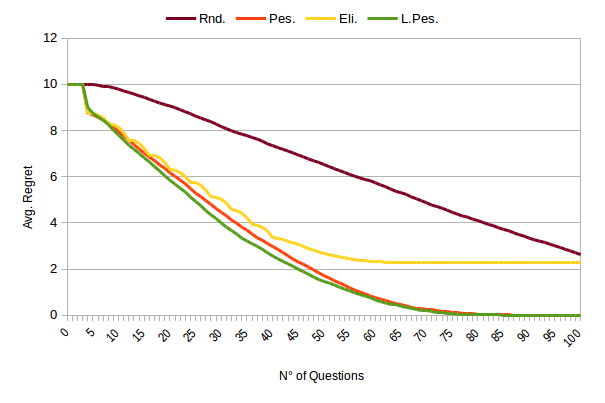
\includegraphics[width=.45\textwidth]{comparison.png}
	\caption{Plot in support of \cref{tab:comparison}}
	\label{fig:comparison}
\end{figure}

\begin{figure}
	\centering
	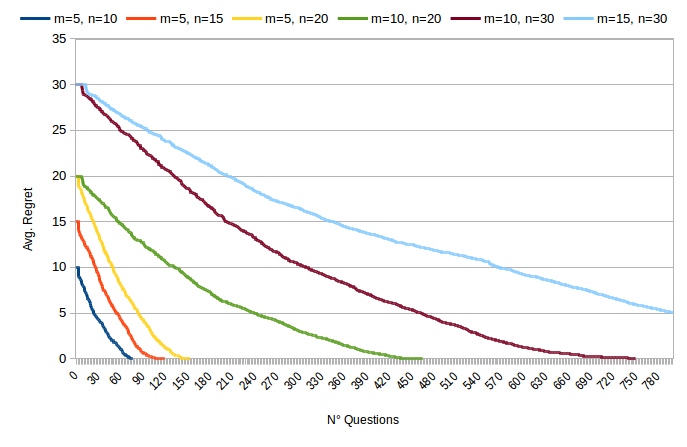
\includegraphics[width=.45\textwidth]{linearity.png}
	\caption{Average $\MMR$ after $k$ questions with Pessimistic strategy after 10 runs for different problem sizes.}
	\label{fig:linearity}
\end{figure}

\begin{table}
	\begin{center}
		\begin{tabular}{S[table-figures-integer=1, table-number-alignment = center, table-figures-decimal=0]S[table-figures-integer=1, table-number-alignment = center, table-figures-decimal=0]S[table-number-alignment = center]S[table-figures-integer=1, table-number-alignment = center, table-figures-decimal=0]S[table-figures-integer=1, table-number-alignment = center, table-figures-decimal=0]}
			\toprule
			{m} & {n} & {$\frac{n}{10}$} & {$k_{\MMR}$} & {$m\cdot n +m^?$} \\
			\midrule
			5 & 10 & 1.0 & 60 &  \\
			5 & 15 & 1.5 & 80 &  \\
			5 & 20 & 2.0 & 110 &  \\
			10 & 20 & 2.0 & 340 &  \\
			10 & 30 & 3.0 & 527 &  \\
			15 & 30 & 3.0 &  &  \\
			\bottomrule
		\end{tabular}
	\end{center}
	\caption{Number of questions needed by Pessimistic strategy to reach $\MMR=\frac{n}{10}$ (represented by $k_{\MMR}$), for different problem sizes.}
	\label{tab:linearity}
\end{table}

We test our strategies using randomly generated datasets. 
Our first goal is to see, with a small problem size ($m = 5, n = 5$) and the (time consuming) Pessimistic strategy, if an important lowering of the maximal regret can be achieved with a reasonable number of questions. We also want to estimate how “hard” such a problem is, by using the Random strategy as a baseline. Third, we want to estimate the loss (in terms of worst regret) when switching to the faster Limited pessimistic strategy. Fourth, we want to see, on a bigger problem size ($m = 10, n = 20$), how many questions must be asked for that strategy to achieve a significant reduction of the worst regret. Finally, we want to evaluate, thanks to the Two phases strategy, the impact of varying the proportion of questions asked to the agents (with respect to questions asked to the chair) on the reduction of the worst regret.
%We also want to see how realistic our approach is for various problem sizes, by estimating the number of questions we would have to ask before being able to reduce the worst regret significantly.

The results are displayed in \cref{tab:comparison,fig:linearity,tab:twoP}, where strategies are designated by Rnd for Random, Pes. for Pessimistic, L.\ pes. for Limited pessimistic and 2 ph. for Two phases. 

We observe that the Pessimistic strategy is able to reduce the regret almost completely after $30$ questions. We also see that Limited pessimistic performs almost as well as Pessimistic; this is good news since (for $m=5$ and $n=5$), the former strategy is much faster and takes only $2.6s$ for a complete elicitation session, while the latter takes $16s$.
%However, it takes $1000$ times more time than the \strat{Random} strategy ($16s$ of the Pessimistic compared to $0.014s$ of the Random). Moreover, the results of the \strat{Limited pessimistic}, that takes almost $80\%$ less of the time of the \strat{Pessimistic} ($2.6s$), are essentially the same.
%In Table \ref{fig:1020}, we can see the drop of regret using a bigger instance.
%Finally in Table \ref{fig:p}
%
%\begin{table}
%	\begin{center}
%		\begin{tabular}{S[table-figures-integer=3, table-number-alignment = right, table-figures-decimal=0]S[table-number-alignment = right]@{ ± }S[table-number-alignment = left]S[table-number-alignment = right]@{ ± }S[table-number-alignment = left]S[table-number-alignment = right]@{ ± }S[table-number-alignment = left]S[table-number-alignment = right]@{ ± }S[table-number-alignment = left]}
%			\toprule
%			{p} & {Comm. Fst.} & {sd} & {Vot. Fst.} & {sd} \\
%			\midrule
%			0 & 0.48 &0.59 & 0.48 &0.59  \\
%			50 & 0.01 & 0.04& 0.0 & 0.0 \\
%			100 & 0.04 & 0.09 & 0.13 & 0.35 \\
%			150 & 0.68 & 0.65 & 0.66 & 0.77 \\
%			200 &   &  &  &  \\
%			250 & 3.2 & 1.67 & 4.07	& 1.51 \\
%			300 &&&& \\
%			350 &&&& \\
%			400 &&&& \\
%			450 &&&& \\
%			500 &&&& \\
%			\bottomrule
%		\end{tabular}
%	\end{center}
%	\caption{Average regret in problems of size $(10, 20)$ after $500$ questions and $10$ runs. Where $p$ represents the number of questions asked to the chair.}
%	\label{tab:twoP500}
%\end{table}

\begin{table}
	\begin{center}
		\begin{tabular}{S[table-figures-integer=3, table-number-alignment = right, table-figures-decimal=0]S[table-number-alignment = right]@{ ± }S[table-number-alignment = left]S[table-number-alignment = right]@{ ± }S[table-number-alignment = left]S[table-number-alignment = right]@{ ± }S[table-number-alignment = left]S[table-number-alignment = right]@{ ± }S[table-number-alignment = left]}
			\toprule
			{p} & {Com. Fst.} & {sd} & {Vot. Fst.} & {sd} \\
			\midrule
			0 & 0.66 & 0.67 & 0.65 & 0.65  \\
			50 & 1.23 & 1.46 & 0.8 & 0.79 \\
			100 & 2.03 & 1.56 &  &  \\
			150 & 3.41 & 1.79 & 4.07 & 1.51 \\
			200 &   &  &  &  \\
			250 & 8.4 & 1.86 & 	& \\
			300 &&&& \\
			350 &&&& \\
			400 &&&& \\
			\bottomrule
		\end{tabular}
	\end{center}
	\caption{Average $\MMR$ in problems of size $(10, 20)$ after $400$ questions and $10$ runs. Where $p$ represents the number of questions asked to the chair. (The $\MMR$ after 400 questions with Pessimistic is $0.62$ ± $0.56$)}
	\label{tab:twoP400}
\end{table}

\section{Conclusions}  
\label{sec:conclusions}
%TODO balance columns appropriately before submitting
%\balance
In this paper we have considered a social choice setting with partial information about the agent's preferences and a partially specified voting rule.
In this setting, we have proposed the use of minimax regret both as a means of robust winner determination as well as a guide to the process of simultaneous elicitation of preferences and voting rule.
Our experimental results %on randomly generated and real world data sets 
suggest that regret-based elicitation is effective and allow to quickly reduce worst regret significantly.
%regret, but they also show that starting with zero knowledge became a pretentious approach really quickly when increasing the size of the problem. Future works will therefore include the test of these strategies on partial specified profiles, ideally on real datasets. An other important direction is the extension to voting rules beyond scoring rules.
%Regret-based elicitation allows to determine near-optimal winners using only few information about the agent preferences.

As part of the contribution of this work, we publish an open-source library that allows to reproduce our experiments, and more (url not displayed for anonymity reasons).

We mention some directions for future works.
Further development of elicitation strategies, considering alternative heuristics, is an important direction. 
Second, elicitation could be extended to voting rules beyond scoring rules.
Finally, an important direction of extension aims at studying how to elicit preferences while restraining to concrete and easy questions.
% Acknowledgements: We thank the reviewers for comments helping to improve the paper. 

%%%%%%%%%%%%%%%%%%%%%%%%%%%%%%%%%%%%%%%%%%%%%%%%%%%%%%%%%%%%%%%%%%%%%%%%

%%% The acknowledgments section is defined using the "acks" environment
%%% (rather than an unnumbered section). The use of this environment 
%%% ensures the proper identification of the section in the article 
%%% metadata as well as the consistent spelling of the heading.

%\begin{acks}
%If you wish to include any acknowledgments in your paper (e.g., to 
%people or funding agencies), please do so using the `\texttt{acks}' 
%environment. Note that the text of your acknowledgments will be omitted
%if you compile your document with the `\texttt{anonymous}' option.
%\end{acks}

%%%%%%%%%%%%%%%%%%%%%%%%%%%%%%%%%%%%%%%%%%%%%%%%%%%%%%%%%%%%%%%%%%%%%%%%

%%% The next two lines define, first, the bibliography style to be 
%%% applied, and, second, the bibliography file to be used.
%\bibliographystyle{abbrvnat} 
%\bibliography{biblio}

\bibliographystyle{ACM-Reference-Format} 
%TODO remove this when submitting, and consider solving the vertical overflows
\vfuzz=5pt
\bibliography{biblio}
\end{document}

%%%%%%%%%%%%%%%%%%%%%%%%%%%%%%%%%%%%%%%%%%%%%%%%%%%%%%%%%%%%%%%%%%%%%%%%

\appendix
\import{preamble/}{appendix.tex}


%%%%%%%%%%%%%%%%%%%%%%%%%%%%%%%%%%%%%%%%%%%%%%%%%%%%%%%%%%%%%%%%%%%%%%%%



